Soit $f$ une fonction définie sur $]0\ ;\ +\infty[$.

On a tracé dans le repère ci-dessous la courbe $C_f$ représentative de la fonction $f$ et la droite $T_A$ tangente à la courbe $C_f$ au point $A$ de coordonnées $(1\ ;\ 20)$.

La droite $T_A$ passe par le point $B$ de coordonnées $(3\ ;\ 10)$.


\begin{center}
	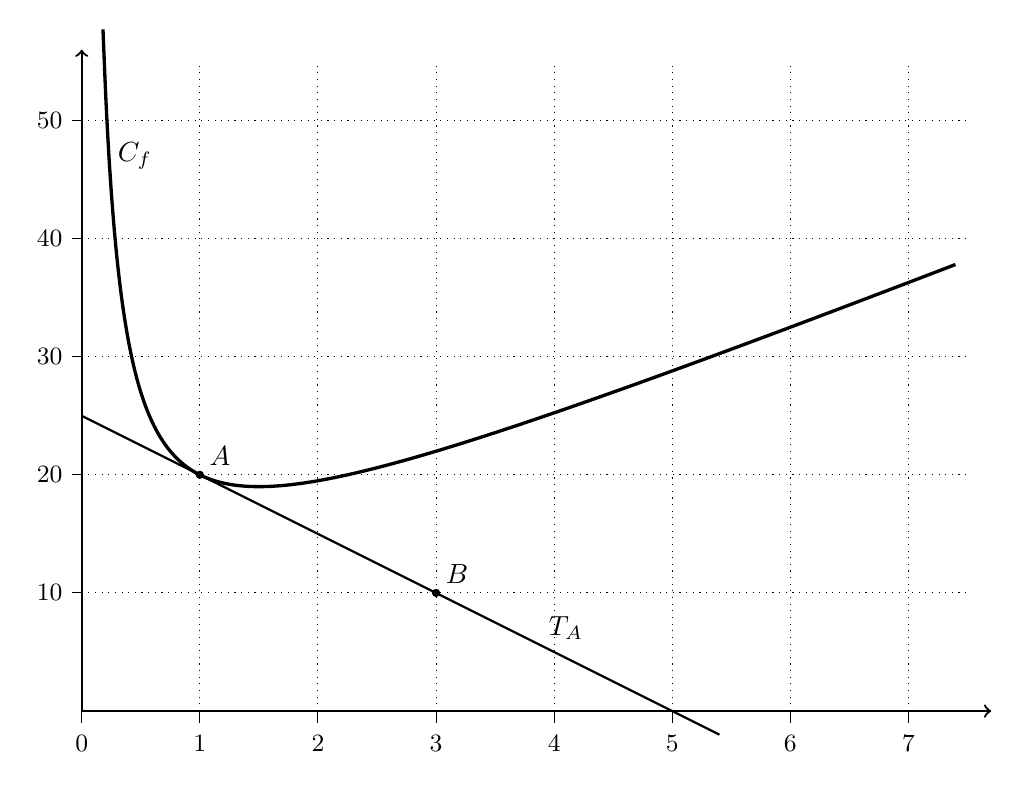
\begin{tikzpicture}[x=1.5cm,y=0.15cm]
		
		
		
		
		
		\foreach \x in {0,1,2,3,4,5,6,7}
		{
			\draw[dotted] (\x,0) -- (\x,55);
		}
		
		
		\foreach \y in {0,10,20,30,40,50}
		{
			\draw[dotted] (0,\y) -- (7.5,\y);
		}
		
		
		\draw[->,thick] (0,0) -- (7.7,0);
		\draw[->,thick] (0,0) -- (0,56);
		
		
		\foreach \x in {0,1,2,3,4,5,6,7}
		{
			\draw (\x,0) -- (\x,-1);
			\node[below] at (\x,-1.2) {\small $\x$};
		}
		
		
		\foreach \y in {10,20,30,40,50}
		{
			\draw (0,\y) -- (-0.08,\y);
			\node[left] at (-0.08,\y) {\small $\y$};
		}
		
		
		\draw[very thick, domain=0.18:7.4, samples=300, smooth, variable=\x]
		plot ({\x},{(4*\x*\x+7*\x+9)/\x});
		
		
		\draw[thick, domain=0:5.4, samples=2, variable=\x]
		plot ({\x},{-5*\x+25});
		
		
		\fill (1,20) circle (1.5pt);
		\fill (3,10) circle (1.5pt);
		
		
		\node[above right] at (1,20) {$A$};
		\node[above right] at (3,10) {$B$};
		\node at (0.45,47) {$C_f$};
		\node at (4.1,7) {$T_A$};
		
	\end{tikzpicture}
\end{center}

\begin{enumerate}
\item \begin{enumerate}
\item Donner $f(1)$.
\item Déterminer la valeur de $f'(1)$.
\item Justifier que l'équation réduite de la tangente $T_A$ à $C_f$ au point $A$ est :
\[
y=-5x+25.
\]
\end{enumerate}
\end{enumerate}

Pour la suite de l'exercice, la fonction $f$ est définie sur $]0\ ;\ +\infty[$ par $f(x)=\dfrac{4x^2+7x+9}{x}$.

On admet que $f$ est dérivable sur cet intervalle.

\begin{enumerate}
\setcounter{enumi}{1}
\item \begin{enumerate}
\item Démontrer que pour tout $x\in]0\ ;\ +\infty[$, on a $f'(x)=\dfrac{(2x-3)(2x+3)}{x^2}$.
\item Étudier le signe de $f'(x)$ sur $]0\ ;\ +\infty[$.
\item En déduire les variations de la fonction $f$ sur $]0\ ;\ +\infty[$.
\end{enumerate}
\item Existe-t-il une tangente à $C_f$ parallèle à la droite d'équation $y=3x+5$ ?

Justifier votre réponse.
\end{enumerate}
